\documentclass[12pt]{article}
\input{/home/tritlo/Dropbox/Latex/header.tex}

\nonums

\title{Tölvugrafík\\Verkefni 3}
\author{Matthías Páll Gissurarson\\mpg3@hi.is}

\lstset{language=JavaScript}
\begin{document}
\maketitle

Verkefnið má finna á slóðinni \url{http://webgl.mpg.is/v2/butterfly.html}, en einnig í meðfylgjandi zip skjali. Ég ætla ekki að hafa neinn kóða í skýrslunni, en hann má finna allan í zip skjalinu.

Við útfærslu er notast er við Cube.js klasan sem gerður var fyrir síðasta verkefni, og með honum voru fiðrildin gerð, en þau eru útfærð í skránni Butterfly.js.
Butterfly klasinn hefur umsjón með að hreyfa og snúa hverju fiðrildi, en einnig að blaka vængjunum. Hægt er að tilgreina hver stefna fiðrildis á að vera,
en þá er reiknað út hver snúningurinn á því þarf að vera.


Hjarðhegðunin er útfærð í flockDir fallinu í butterflies.js.
Þar byrjum við að finna hvaða fiðrildi við eigum að skoða, með því
að finna þau fiðrildi sem eru nógu nálægt til að fylgjast með, og eru nógu litlu
horni frá sjónstefnu fiðrildisins sem við erum að breyta stefnunni fyrir.

Ef fiðrildið sem verið er að skoða uppfyllir skilyrðin, þáer því bætt við í listann af fiðrildum sem skoða á.
Yfir þennan lista (þ.e. fiðrildi sem skoða á) er svo reiknuð meðalstaðsetning og stefna, en einnig sérstaklega meðalstefna þeirra
fiðrilda sem eru of nálægt.
``Of nálægt'', ``nógu nálægt'' og ``nógu litlu horni'' er allt eitthvað sem er skilgreint með parametrum í upphafi skjals.

Ný stefna fiðrildis er svo reiknuð sem normalíseruð línuleg samantekt þessara þátta, þ.e. stefna að meðalstaðsetningu, stefna frá meðalstaðsetningu þeirra sem eru of nálægt og meðalstefna nágranna. Nýju stefnunni er skilað úr því falli, en hún er svo notuð til að uppfæra stefnu fiðrildisins. Vægi hvers þátts má stilla með slider-um sem eru fyrir neðan.

Þegar þetta var svo keyrt fannst mér sum fiðrildin vera að skipta sífellt um stefnu,
en það fannst mér óþægilegt. Því setti ég inn tímateljara, en stefna fiðrildis er bara
uppfærð ef nógu langt er síðan stefna þess var uppfærð síðast (``ákvörðunar tími'').
Sá tími er randomize-aður fyrir hvert fiðrildi, en einnig er upphafshraða, staðsetningu,
blakvinkli vængja og blakhraða randomize-að.

Í upphafi eru búin til þó nokkuð mörg fiðrildi, en notandi getur svo bætt við fleirum ef hann vill.
Einnig er hægt að stjórna sjónarhorninu með músinni, en skrunhjólið leyfir manni að ``zoom-a'' inn og út.

\begin{figure}[H]
  \centering
  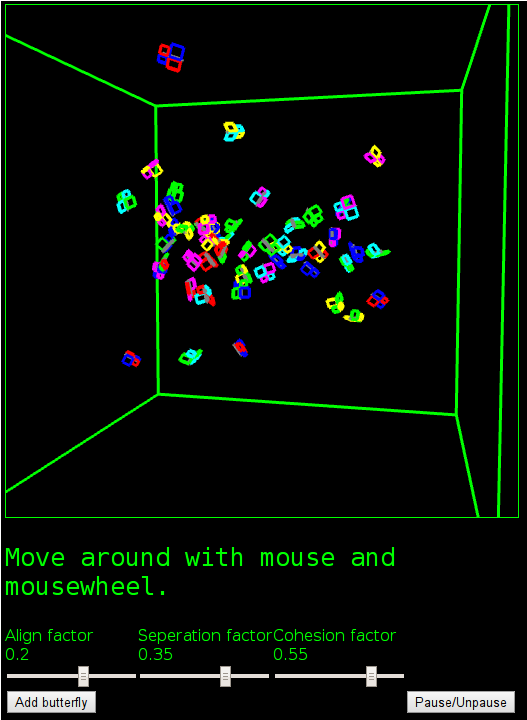
\includegraphics[width=9cm]{butterfly.png}
  \caption{Skjáskot af hermuninni.}
  \label{fig:butterfly}
\end{figure}
\begin{figure}[H]
  \centering
  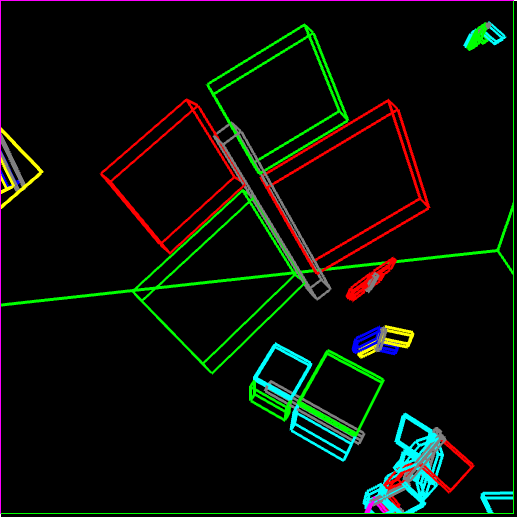
\includegraphics[width=12cm]{butterfly2.png}
  \caption{Nærmynd af fiðrildi}
  \label{fig:butterfly2}
\end{figure}

\end{document}